% Chapter Template

\chapter{Methodology} % Main chapter title

\label{Chapter3} % Change X to a consecutive number; for referencing this chapter elsewhere, use \ref{ChapterX}

\lhead{Chapter 3. \emph{Methodology}} % Change X to a consecutive number; this is for the header on each page - perhaps a shortened title

%----------------------------------------------------------------------------------------
%\tSECTION 1
%---------------------------------------------------------------------------------------
\section{System Overview}

The core of this project is the integration of a powerful vision-based scene understanding model (BEVDepth) with a state-of-the-art motion forecasting model (AgentFormer). The hypothesis is that the rich, dense visual context provided by BEVDepth can enhance AgentFormer's ability to predict future trajectories of agents in a scene. This section details the architecture of the integrated system and the methodology used for its implementation.

Figure \ref{fig:system_overview} presents a high-level overview of the integrated model. The system consists of two main components: the BEVDepth model for feature extraction and the AgentFormer model for motion forecasting.

\begin{figure}[h]
\centering
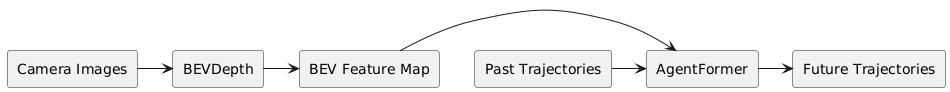
\includegraphics[width=0.8\textwidth]{system_overview.png}
\caption{High-level overview of the integrated BEVDepth and AgentFormer model.}
\label{fig:system_overview}
\end{figure}

The workflow is as follows:
\begin{enumerate}
    \item The BEVDepth model takes a sequence of camera images as input and generates a dense Bird's-Eye-View (BEV) feature map of the scene.
    \item The AgentFormer model takes the past trajectories of agents in the scene as input.
    \item The BEV feature map is then fused with the agent's trajectory information within the AgentFormer model.
    \item The fused representation is used by AgentFormer's transformer-based architecture to predict the future trajectories of the agents.
\end{enumerate}

The following sections provide a more detailed description of each component and the integration process.

\section{Experimental Setup}

The experiments for this thesis were conducted on a high-performance computing setup. The system was equipped with a 300GB solid-state drive (SSD) for fast data access, which is crucial for handling the large nuScenes dataset. For model training and inference, an NVIDIA RTX 5090 GPU with 32GB of VRAM was used. This powerful GPU enabled the training of deep learning models with large batch sizes and high-resolution inputs.

\section{Integration with AgentFormer}

The integration of the BEV features into the AgentFormer model is handled within the {\sloppy\texttt{AgentFormer/model/agentformer.py}} file. The core logic resides in the `AgentFormer` and `ContextEncoder` classes.

\subsection{AgentFormer Model}

The `AgentFormer` class's {\sloppy\texttt{\_\_init\_\_}} method checks for the {\sloppy\texttt{use\_bev}} flag in the configuration. If it is set to `True`, the following actions are taken:

\begin{enumerate}
    \item The `BaseLSSFPN` class from {\sloppy\texttt{model/bev/base\_lss\_fpn.py}} is imported and used to initialize the BEV encoder ({\sloppy\texttt{self.bev\_encoder}}).
    \item A fusion module, {\sloppy\texttt{self.bev\_fusion\_module}}, is created. This is a simple Multi-Layer Perceptron (MLP) designed to fuse the BEV features with the agent's trajectory features.
\end{enumerate}

In the `forward` pass of the `AgentFormer` model, the BEV features are either loaded from pre-computed files or extracted on-the-fly by the {\sloppy\texttt{bev\_encoder}}. These features are then passed to the `ContextEncoder`.

\subsection{Context Encoder}

The `ContextEncoder` is responsible for encoding the past trajectories of the agents. The integration of BEV features happens in its `forward` method.

\begin{enumerate}
    \item The method checks if a {\sloppy\texttt{bev\_feature\_map}} is available in the input data.
    \item If BEV features are present, the model samples features from the BEV map at the 2D location of each agent for each timestep in its past trajectory. This is achieved using the {\sloppy\texttt{grid\_sample}} function from PyTorch, which allows for differentiable sampling from a feature map.
    \item The sampled BEV features are then concatenated with the agent's existing trajectory features (e.g., position, velocity).
    \item The concatenated features are passed through the \texttt{bev\_fusion\_module} (the MLP) to produce a fused feature vector.
    \item This fused feature vector is then used as the input to the AgentFormer's transformer encoder, allowing the model to reason about the agent's future motion based on both its past trajectory and the surrounding visual context from the BEV map.
\end{enumerate}

This methodology allows for a tight integration of visual and trajectory information, with the goal of improving the accuracy of motion forecasting. The following chapter will present the results of this integration and analyze the reasons for the observed performance.
